%
% File acl2015.tex
%
% Contact: car@ir.hit.edu.cn, gdzhou@suda.edu.cn
%%
%% Based on the style files for ACL-2014, which were, in turn,
%% Based on the style files for ACL-2013, which were, in turn,
%% Based on the style files for ACL-2012, which were, in turn,
%% based on the style files for ACL-2011, which were, in turn, 
%% based on the style files for ACL-2010, which were, in turn, 
%% based on the style files for ACL-IJCNLP-2009, which were, in turn,
%% based on the style files for EACL-2009 and IJCNLP-2008...

%% Based on the style files for EACL 2006 by 
%%e.agirre@ehu.es or Sergi.Balari@uab.es
%% and that of ACL 08 by Joakim Nivre and Noah Smith

\documentclass[11pt]{article}
\usepackage{acl2015}
\usepackage{times}
\usepackage{url}
\usepackage{latexsym}
\usepackage{graphics}
\usepackage{amsmath}
\usepackage[table,xcdraw]{xcolor}
\usepackage[pdftex]{graphicx}
\usepackage[english]{babel}
\usepackage{geometry} 
\usepackage[utf8]{inputenc}
\usepackage{graphicx}
\usepackage{movie15}
\usepackage{fancyhdr} 
\usepackage{listings}
\usepackage[hidelinks]{hyperref}
\hypersetup{
%	colorlinks,
	citecolor=white,
	filecolor=white,
	linkcolor=white,
	colorlinks=false,
	urlbordercolor=white,
	citebordercolor=white,
	linkbordercolor = red
}
%\setlength\titlebox{5cm}

% You can expand the titlebox if you need extra space
% to show all the authors. Please do not make the titlebox
% smaller than 5cm (the original size); we will check this
% in the camera-ready version and ask you to change it back.


\title{Prediction of User Appreciation of Yelp's Businesses Based on Text Reviews Hidden Features}
\author{Umberto Di Fabrizio \\
	University of Illinois at Chicago\\
	{\tt udifab2@uic.edu} \\\And
	Vittorio Selo \\
	University of Illinois at Chicago\\
	{\tt vselo2@uic.edu} \\}


\date{}

\begin{document}
\maketitle
\begin{abstract}
	This work aims to predict the vote (i.e.stars) that an user gives to a business on Yelp. Each user is modeled by a set of his most important words, which are extracted from his reviews and his \textit{tastes} are used to predict how much he will like a business. The contribution given by this work are: 1) A new framework is build to profile the users' tastes based only on the text in his reviews 2)The user profiling algorithm is used to predict the likelihood that the user likes a business. The method reaches 54\% of accuracy revealing the effectiveness of the approach and encourages further investigation on this area, in particular combining this approach with classical high level features.
\end{abstract}

\section{Introduction}

Nowadays with the growth of websites that offer user-generated content (e.g. Yelp, IMDb, TripAdvisor) there is an increasing need, for companies, to extract the tastes of the users in order to make unique the user experience.\\
For this reason, recently, there have been a lot of researches in this area aimed to increase the effectiveness of the contents provided to the user (e.g. Netflix competition\cite{Netflix}, Amazon, Yelp\cite{Nikulin}).
The traditional approach is based on a system that tries to predict the rating that a user would give to an item, this type of engines are called recommendation systems and have gained popularity in the recent years.\\
Generally to achieve this outcome the system is trained using high-level features, for instance in a movie platform those features would be: the rating of the film, the genre, the actors and so on.\\
Those characteristics are easily obtained from the database and are extensively used.\\
Our aim is to extract \textit{hidden-features} of an user in order to understand their personal tastes and extract this information only by the text reviews.
We call \textit{hidden-features} those personal tastes of an user which can even be unconscious for the user himself. 
For example suppose a user writes reviews of Mexican restaurants, why is one restaurant better than another although the food is good in both? Usually, people pay attention to details such as lights, atmosphere, the type of customers and so on, and sometimes without even being aware of their pet peeves.\\
The issue is \underline{how} to find out, in an automatic way, those tastes that rule people feelings about a place (or an item) and \underline{which} source to use.\\

To extract the \textit{hidden-features} we will mine the reviews of an user in order to collect the most common topics (furniture, lights, etc.) and  understand what he really observes to judge a business (e.g. restaurant, pub, hotel).
The hypothesis is that if an user always talks about certain topics then he cares a lot about that theme and this can guide the recommendation system.\\
Once the user hidden features are extracted we use them to train an ensemble of classifiers (SVM, Naive Bayes, Linear Regression) that learn how to predict the starts vote by those features.\\
We develop two methods: the first one is composed by one classifier that predicts one of the 9 possible classes (i.e. \{1, 1.5, 2, 2.5, 3, 3.5, 4, 4.5, 5\}) the second method is composed by three classifier which independently predict three subsets of the classes (i.e. \{1, 1.5 ,2\},\{2.5 ,3 ,3.5\},\{4, 4.5, 5\}) and then trains a Adaptive Boosting classifier on the predictions of those three preceding classifiers to obtain the final prediction.\\
The approach developed has the strength that it does not make any assumption on the type of reviews, user or platform, nor it make use of any specific domain-knowledge, this makes the framework highly flexible and ready to be used across different platform with no changes.

\section{RELATED WORK}

The classical approach based on user behavior and ratings is the one exploited by \cite{Nikulin}, in his work the collaborative filtering approach is combined with the content-based filtering to create an Hybrid Recommender System. A collaborative filtering approach build a model from a user's
past behavior as well as similar decisions made by
other users whilst the content-based filtering approaches
utilize a series of discrete characteristics of an item in order to recommend
additional items with similar properties. The approach works pretty good by it completely ignores text reviews from users which express the reason why a user has bought a certain item.
The idea to address the user profiling by exploiting the text reviews is quite knew in the literature,because it is a hard task and because the existing methods are mainly based on users ratings and ignore text reviews.The common approach is the one by \cite{Dupuy} where meaningful words are filtered from a database of text reviews then the topics are extracted using LDA and finally a similarity measure is used to score the similarity between topics and based on the result the user receives a certain suggestion.\\
The main problem with user reviews on Yelp is that there is a great percentage of them which is fake, infact almost 1 out of 5 review is marked as fake by the Yelp's algorithm. As demonstrated in the work by \cite{Luca} economic incentives are a heavy factor into the decision to commit fraud. Moreover they show that , a restaurant
is more likely to commit review fraud when its reputation is weak and this may explain the highly skewed distribution of ratings of Yelp's review that we have to face.
We took inspiration from the work by \cite{McAuley}, the basic idea is to exploit the richness of information in the text reviews to extract topics. They develop statistical models that combine
latent dimensions in rating data with topics in review text moreover they combine ratings with review text and predict
ratings more accurately than approaches that consider either of the
two sources in isolation.
Our approach tries to dig deeper in the user profiling, with the purpose to find those unique characteristics of the user and to suggest a business that he will surely like. To follow this idea we decided not to use LDA but to extract frequent words in a  user reviews and use them as indicators for user tastes.\\
\section{DATA}
We have used the Yelp dataset\cite{yelp} which is right now freely available because of the Yelp challenge that is currently ongoing.\\
The dataset is composed by 1.6M reviews and 500K tips by 366K users for 61K businesses and spans across several cities( Edinburgh, Karlsruhe
, Montreal, Waterloo, Pittsburgh, Charlotte, Urbana-Champaign, Phoenix, Las Vegas, Madison).\\
Because of the dimensions of the dataset and the computational power we have access to, we decided to limit our investigation to businesses in the area of Edinburgh(23780 reviews, 3150 users,4576 businesses). Anyway this work can be easily generalized to the all dataset or virtually to any dataset with the same info.\\
The format of the dataset is shown in fig ~\ref{review}.
\begin{figure}[thpb]
	%\centering
	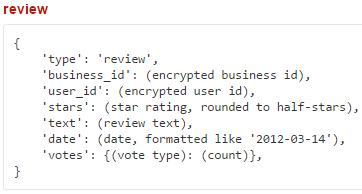
\includegraphics[scale=0.75]{img/review.png}
	\caption{Yelp's Dataset review format.}
	\label{review}
\end{figure}
\section{METHODS}
\subsection{PREPROCESSING}
The reviews of Edinburgh businesses are tokenized using the tweeter tokenizer (keeps smilies ':)'), then we use the nltk package for python trained on the  Penn Tree Bank dataset for the POS-tagging.\\
For our first approach we scan each user's reviews, we remove stop-words and detect the nouns that he uses finally for each noun we collect three features.
Let M be the set of all users, R the set of all reviews.
Given user m $\in$ M let $r_m$ be the set of all reviews of user m then define $X_m$ as the set of all nouns of the user m.
Let $n_{xmz}$ be the number of times that the word x belonging to $X_m$ appear in review z $\in$ $r_m.$
Let $s_{mz}$ be the rank that user m gave to review z.\\
Now we can define:
\begin{itemize}
	\item \textbf{Frequency}: frequency of that noun compared to the other nouns used\\
	i.e. how much the user talks about X?
	\[ f(x,m)= \frac{\sum_{i \in r_m}n_{xmi}}{\sum_{i \in r_m}\sum_{k \in X_m} n_{kmi}} \]
	\item \textbf{Regularity}: how constantly is that noun used in the reviews\\
	i.e. does the user talks about X in most of the reviews or not?
	\[ r(x,m)= \frac{\sum_{i \in r_m}
		n_{xmi}  \frac{1}{\sum_{k \in X_m}n_{kmi}}}	
	{|r_m|} \]
	\item \textbf{Relevance}: how influent is the noun to predict the rank?\\
	i.e. is X important to the final business score?
	\[ i(x,m)= \frac{\sum_{i \in r_m}
		n_{xmi}  \frac{s_{mi}}{\sum_{k \in X_m}n_{kmi}}}	
	{|r_m|} \]
\end{itemize}
As shown in the formulas above all the scores are normalized, in this way we avoid any biasing problem for the classifier.\\
\subsection{FIRST METHOD}
The pipeline for our first method is shown in figure ~\ref{first},
\begin{figure}[thpb]
	%\centering
	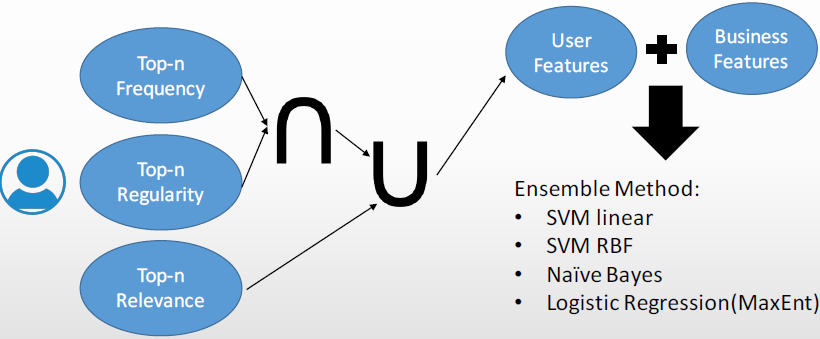
\includegraphics[scale=0.32]{img/firstMethod.png}
	\caption{First Method pipeline.}
	\label{first}
\end{figure}	
for each user we extract nouns, adverbs and adjectives and for each of them 
 we have the 3 features. We select the top n (30) based on frequency and we intersect them with the top 30 based on regularity, this is because we want words that are frequent AND regular, finally we compute the union between those words and the top 30 based on relevance, this is because the influence of a word to the rank is fundamental by itself. 
We run the same algorithm to collect words and their features for the businesses, scanning all the reviews of a business.
In the end for each user we have his\textit{ best words} with their relative 3 hidden-features and for each business we have its words with their 3 hidden-features. For each best word of a user we look in the business best words to check if there is a match, in this case the business values for that word are collected otherwise a default $[0,0,0]$ is assigned.
In the end we have a vector:\\
$[$ User best nouns $]  [$ Business word in common with user $]$\\
for each user-business couple.
The length of the features vector is $2 * |\text{best user noun}|$, thus the input to the classifier is between $(30*3)*2=180$ and $(60*3)*2=360$.\\\\
The pairs for user features and business features are then used to train an ensemble classifier which predicts the final score of a business.
For each user we trained an ensemble of classifiers, the validation set has been used to choose the best classifier for each user among Naive Bayes, SVM (radial basis function kernel) and Logistic Regression (MaxEnt).
\subsection{SECOND METHOD}
The workflow for our second method in shown in figure ~\ref{second}.
\begin{figure}[thpb]
	%\centering
	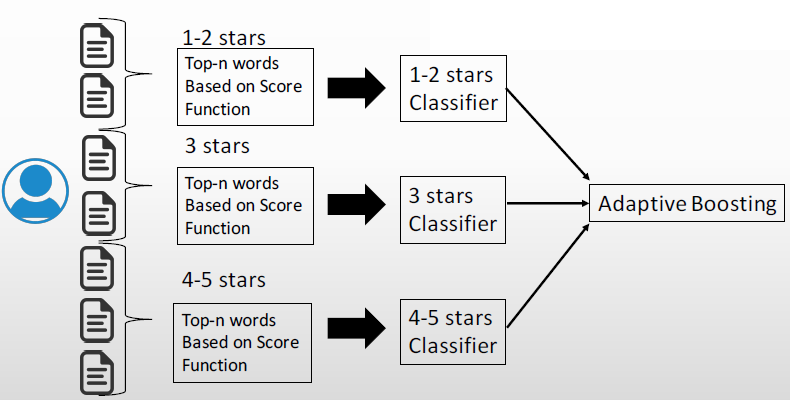
\includegraphics[scale=0.35]{img/secondMethod.png}
	\caption{Second Method pipeline.}
	\label{second}
\end{figure}	
For our second approach we identified three subset based on the users' review stars [1-2], [3], [4,5]. The reason is that we need an algorithm that can distinguish classes '1' and '2' from the rest of the world as well as discriminate between class '4' and '5'. For each subset we used two features: frequency and regularity (we omit relevance because in this context is not meaningful) and we ranked the words accordingly to the score:\[ S=log(frequency)+log(regularity) \]
This measure takes into account both features and avoids underflow.
We extracted the 100 most important nouns (or less if there were not enough) for each of those subsets.\\
As in the first approach we applied the same algorithm to the businesses and then we extracted the business nouns in common with the user.\\
For each subset of user's review we train a classifier which is particularly good at discriminate between only a subset of classes (e.g. '3' or 'Other').//

We selected users with more than 50 reviews and trained three classifiers as follows (on the right the majority class baseline):
\begin{enumerate}
	\item 1, 2, Other - 91.7\%
	\item 3, Other - 76.8\%
	\item 4, 5, Other - 46.3\%
\end{enumerate}
This is motivated by the fact that we need to discriminate very well between 4 and 5,and to avoid to bias the classifier towards the majority class.\\
Again it appears that the first classifier has an high accuracy, anyway it mostly predict the 'Other' class because of the unbalanced dataset.\\
Each of those classifier is actually an ensemble made by SVM(rbf kernel) and MaxEnt, the best classifier is chosen with the results on the validation test by extracting which classifier performs better with respect to the different number of minimum reviews (e.g. the users with reviews between 20 and 40 are best classified by the SVM whilst the MaxEnt is better to predict users with more than 40 reviews).\\
Finally we combine the predictions of each of this three classifiers to train an Adaptive Boosting algorithm with a Decision Tree base estimator that predicts the final rank of a review ([1,..,5]).\\
\subsection{EXPERIMENTS SETUP}
For our first method we selected all the user with more than 20,25,50,75 reviews and compared results. The random baseline is theoretically 1/9 = 11.1\% but in our dataset there are not half stars reviews so the classes to predict are only 5 (i.e.\{1,2,3,4,5\}) which raises the random baseline to 20\%.
A more meaningful baseline takes into account the distribution of stars in the dataset and always predicts the majority class ('4'), in this case the accuracy is 42.3\%.
  The highest baseline is actually the user majority class which predicts the user average stars vote for any business in the user test (e.g. if a business rank given by an user is on average 3 we always predict 3 for that user), this raises the baseline to 44.9\%.\\
Fig ~\ref{histStars} reveals how skewed is the curve of rankings on Yelp, in fact the number of 4 and 5 stars by them selfs are 69.2\% of the all dataset.
\begin{figure}[thpb]
	\centering
	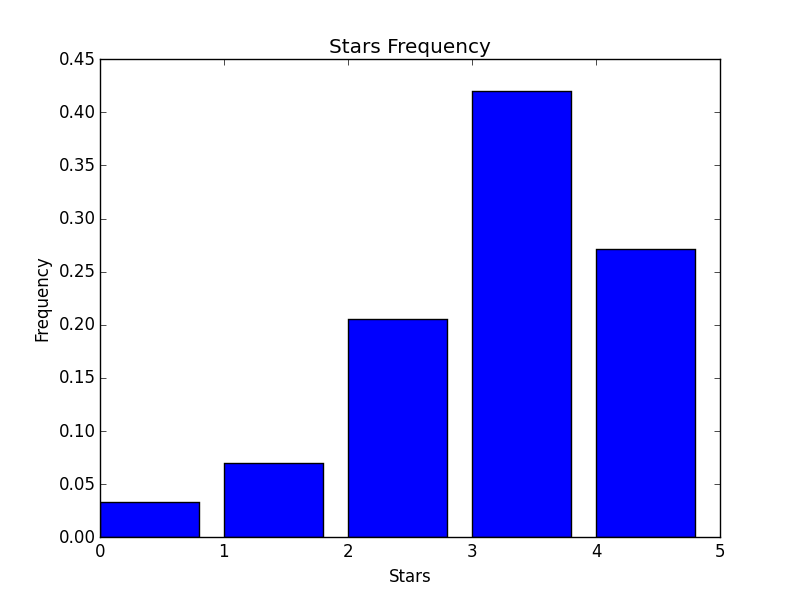
\includegraphics[scale=0.4]{img/starsFrequency.png}
	\caption{Distribution of stars of Yelp Edinburgh dataset.}
	\label{histStars}
\end{figure}
We divided the test between train(80\%), validation set (10\%) and test (10\%).

\section{RESULTS}
The results for the first approach shows that 50 reviews are enough to profile an user, as presented in Table ~\ref{tab}, this reduces the number of user selected to 72.\\
\begin{table}[]

	\caption{Accuracy based on the minimum number of reviews per user}
	\label{tab}
	\begin{tabular}{|c|c|c|c|c|}
		\hline
		Min Rev & 20    & 25    & 50     & 75    \\ \hline
		Baseline    & 0.441 & 0.442 & 0.449  & 0.449 \\ \hline
		Method 1    & 0.445 & 0.446 & 0.455  & 0.451 \\ \hline
		Method 2    & -     & -     & 0.539* & -     \\ \hline
	\end{tabular}
\end{table}
For the second method we achieved a statistical significant improvement reaching 54\% of accuracy\footnote{*p-value$\approx$ 0}. The analysis of the second method has been further divided to understand the accuracy of each of the three classifiers:
fig. ~\ref{class} shows the comparison of each class with respect to its baseline; the approach cannot improve the accuracy of the class [1-2] but it outperform the baseline for the classes [3] and [4-5], especially the accuracy improves more than 12\% for class [4-5].\\
Combining the three prediction with the Adaptive Boosting model we achieve an overall accuracy of 54\% outperforming by 9\% the baseline.
\begin{table}[]
	\centering
	\caption{Accuracy per class}
	\label{class}
	\begin{tabular}{|c|c|c|c|}
		\hline
		Class      & {[}1-2{]} & {[}3{]} & {[}4-5{]} \\ \hline
		Baseline   & 91.7\%    & 76.8\%  & 46.3\%    \\ \hline
		Our method & 91.7\%    & 79.5\%*  & 58.7\%*    \\ \hline
	\end{tabular}
\end{table}
\subsection{Error Analysis}
When dealing with recommendation system it is important to understand how much does the system fails when it does not predict the right class and how does it fail.\\
In the experiments we found out that the baseline majority class has an average error of -0.15, which means that it usually overestimate its prediction, moreover this is by itself a very low error.\\
Our first model has an average error of -0.10 which means that it still overestimates the stars but with less bias.\\
Finally our second model has the lowest average error of -0.08.
Table ~\ref{conf} shows the confusion matrix for method 2: it is really meaningful that our classifier is usually wrong on the adjacent classes which means that, for example, when the true prediction is '4' it predicts '3' or '5' and less frequently '2'. This is very important for a recommendation system because we can trust the fact the the system will always predict something near the true value and not just a random error.
From the confusion matrix we can also see the struggle of the algorithm to predict the classes '1' and '2', this is mainly due to the low number of training samples for those classes and the highly skewed distribution of votes.
\begin{table}[]
	\centering
	\caption{Confusion Matrix, method 2}
	\label{conf}
	\begin{tabular}{|c|r|r|r|r|r|}
		\hline
		True/Predicted & \multicolumn{1}{c|}{1} & \multicolumn{1}{c|}{2} & \multicolumn{1}{c|}{3} & \multicolumn{1}{c|}{4} & \multicolumn{1}{c|}{5} \\ \hline
		1              & 0                      & 5                      & 8                      & 5                      & 4                      \\ \hline
		2              & 1                      & 17                     & 20                     & 43                     & 11                     \\ \hline
		3              & 0                      & 17                     & 144                    & 113                    & 27                     \\ \hline
		4              & 0                      & 22                     & 67                     & 422                    & 66                     \\ \hline
		5              & 0                      & 14                     & 18                     & 153                    & 140                    \\ \hline
	\end{tabular}
\end{table}
\section{CONCLUSION}
The work has presented two methods to profile the users' tastes from the text reviews. The comparison with the baseline shows that the second one increases the accuracy up to 54\%.\\
This demonstrates that it is possible to extract user related information only from the text. The approach is very flexible and can be adopted to any web platform because it does not depend on any domain-specific knowledge.\\
The limitation of our approach is mainly in the fact that the dataset is very biased towards higher scores. For this reason we would like to extend our approach and try to consider a more balanced dataset both by applying stratified sampling or by adopting a different dataset which may be very useful to compare the performances.\\
We would also like to extend the noun extraction by extending each noun with its synonyms and/or hypernym so that the match between user nouns and business nouns can be increased.\\
Finally,the framework that we developed opens the way to several extensions, for instance the sentiment linked to a certain noun can be extracted so that the feeling towards the topic can be added to the features.\\




\addtolength{\textheight}{-12cm}   % This command serves to balance the column lengths
% on the last page of the document manually. It shortens
% the textheight of the last page by a suitable amount.
% This command does not take effect until the next page
% so it should come on the page before the last. Make
% sure that you do not shorten the textheight too much.


%%%%%%%%%%%%%%%%%%%%%%%%%%%%%%%%%%%%%%%%%%%%%%%%%%%%%%%%%%%%%%%%%%%%%%%%%%%%%%%%
\newpage
\section*{APPENDIX}
The work has been evenly distributed between the students who have developed the two methods during several brain storming sessions. In particular Vittorio has worked on the POS-tagging of the dataset and on the implementation of Method 1 while Umberto has implemented the Method 2 and worked on the error analysis.
%Appendixes should appear before the acknowledgment.

%\section*{ACKNOWLEDGMENT}


%%%%%%%%%%%%%%%%%%%%%%%%%%%%%%%%%%%%%%%%%%%%%%%%%%%%%%%%%%%%%%%%%%%%%%%%%%%%%%%%

\begin{thebibliography}{}
	
	
\bibitem[\protect\citename{Yelp} 2015]{yelp}
	Yelp Dataset.
\newblock 2015
	\newblock \href{www.yelp.com/dataset_challenge}{www.yelp.com/dataset\_challenge}
	
\bibitem[\protect\citename{Netflix} 2009]{Netflix}
Netflix Challenge.
\newblock 2009.
\newblock \href{www.netflixprize.com/index}{www.netflixprize.com/index}
	
\bibitem[\protect\citename{Aletras} 2014]{Aletras} %sim
Aletras et al.
\newblock 2014.
\newblock \textit{Measuring the Similarity between Automatically Generated Topics}.

\bibitem[\protect\citename{Nikulin} 2014]{Nikulin} %altroYelp
Vladimir Nikulin.
\newblock 2014.
\newblock \textit{Hybrid Recommender System for Prediction of the Yelp Users}.

\bibitem[\protect\citename{Dupuy} 2014]{Dupuy} %rev
Christophe Dupuy et al.
\newblock 2014.
\newblock \textit{Content Profiling from Text Reviews}.

\bibitem[\protect\citename{Luca, Zervas} 2015]{Luca} %rev
Michael Luca, Georgios Zervas
\newblock 2015.
\newblock \textit{Fake It Till You Make It:	Reputation, Competition, and Yelp Review Fraud}.

\bibitem[\protect\citename{McAuley, Leskovec} 2013]{McAuley} %rev
Julian McAuley, Jure Leskovec.
\newblock 2015.
\newblock \textit{Hidden Factors and Hidden Topics:
	Understanding Rating Dimensions with Review Text}.




\end{thebibliography}

\end{document}